
\documentclass[11pt,a4paper]{article}
\usepackage[utf8]{inputenc}
\usepackage[T1]{fontenc}
\usepackage{lmodern}
\usepackage[a4paper,margin=1in]{geometry}
\usepackage{amsmath,amssymb}
\usepackage{booktabs,array,tabularx}
\usepackage{graphicx}
\usepackage{tikz}
\usetikzlibrary{arrows.meta,positioning,shapes.geometric}
\usepackage{pgfplots}
\pgfplotsset{compat=1.17}
\usepackage[round]{natbib}
\usepackage{hyperref}
\usepackage{caption}
\usepackage{enumitem}
\hypersetup{colorlinks=true,linkcolor=black,citecolor=black,urlcolor=blue}
\setlength{\parindent}{0pt}
\setlength{\parskip}{0.55em}

\title{Reference-Component Extraction from Hebrew-Aramaic Responsa under Low-Resource and Imbalanced Conditions}
\author{Menachem Sperka\\M.Sc. Program in Computer Science, Artificial Intelligence Specialization\\Supervisor: Prof. Yaakov HaCohen-Kerner}
\date{}

\begin{document}
\maketitle

\begin{abstract}
This paper presents a controlled study of reference-component extraction from Hebrew-Aramaic Jewish Responsa literature. The task is formulated as token-level named entity recognition over a small annotated corpus of 300 sentences and approximately 6,800 tokens, with 898 entity tokens and a dominant non-entity class. Four Hebrew transformer encoders are evaluated: DictaBERT, BEREL 3.0, HeRo, and AlephBERT-Gimmel. The study compares sentence-level split strategies, targeted masked-language-model augmentation, regular one-stage NER, a cascaded three-step pipeline, confidence-based fusion, and SVM-based fusion. All comparisons use 20 seed-aligned runs and paired Wilcoxon signed-rank tests. The strongest robust setting is BEREL 3.0 with Multilabel Stratified splitting, augmentation, and SVM Fusion, reaching 0.852 mean F1. A conservative non-router setting, BEREL 3.0 with Multilabel Stratified splitting, augmentation, and Confidence Fusion, reaches 0.848 mean F1. The results show that in small specialized Hebrew-Aramaic corpora, data design and inference design are as important as the choice of pretrained encoder.
\end{abstract}

\textbf{Keywords:} named entity recognition; Hebrew NLP; Responsa literature; low-resource learning; data augmentation; citation extraction; transformer models.

\section{Introduction}
Jewish Responsa literature contains many references to earlier authors, books, chapters, and sections. Extracting these references is useful for digital humanities, legal history, and citation-network analysis \citep{satlow2022,bengigi2025}. This paper focuses on a smaller technical subtask: token-level extraction of the reference components themselves.

The task is challenging because the data is small and imbalanced, the text is Hebrew-Aramaic, and references are often abbreviated or only partially structured. A standard transformer fine-tuning pipeline can produce unstable conclusions in this setting because a single random split may underrepresent rare labels. Therefore, this study asks whether better splitting, targeted augmentation, and fused inference can improve low-resource reference-component NER.

\section{Related Work}
Reference extraction from rabbinic literature is connected to earlier work on biblical quotation identification, dating of rabbinic texts, and citation-network analysis \citep{hacohen2010,moghaz2019,satlow2022}. The closest recent study is \citet{bengigi2025}, which automatically constructs citation networks from medieval Jewish Responsa literature. The present study is complementary: it does not claim a direct benchmark comparison, but analyzes how to train and evaluate reference-component NER when only a small imbalanced annotated dataset is available.

The encoder comparison uses recent Hebrew language models: AlephBERT \citep{seker2022alephbert}, AlephBERT-Gimmel \citep{gueta2023alephgimmel}, HeRo \citep{shalumov2023hero}, DictaBERT \citep{shmidman2023dictabert}, and BEREL for rabbinic-encoded language \citep{shmidman2022berel}. The method design is also related to low-resource NER, sequence constraints, data augmentation, and classifier fusion \citep{li2022ner,nguyen2023auc,zhou2022melm,florian2003,awasthy2020}.

\section{Data and Task}
The final corpus contains 300 annotated sentences, about 6,800 tokens, and 898 entity tokens. Most tokens are labeled \texttt{O}. The entity schema includes author, book, chapter, section, sub-chapter, and prefix markers that introduce these components.

\begin{table}[htbp]
\centering
\small
\caption{Entity distribution in the annotated corpus.}
\label{tab:journal_entity_dist}
\begin{tabular}{lrr}
\toprule
Entity & Tokens & Percent \\
\midrule
\texttt{AUT} & 308 & 34.30 \\
\texttt{BOK} & 180 & 20.04 \\
\texttt{CHP} & 120 & 13.36 \\
\texttt{SCHP} & 58 & 6.46 \\
\texttt{SEC} & 75 & 8.35 \\
\texttt{pCHP} & 81 & 9.02 \\
\texttt{pSCHP} & 54 & 6.01 \\
\texttt{pSEC} & 22 & 2.45 \\
\bottomrule
\end{tabular}
\end{table}

Preprocessing experiments showed that standard tokenization was not sufficient for the corpus because abbreviations and punctuation marks are important for reference boundaries. The final preprocessing used a Hebrew-oriented tokenizer that preserves abbreviations and separates full-stop punctuation from partial-stop punctuation. Abbreviation expansion was evaluated manually on a sample and reached 72.77 percent correct expansions.

\section{Methods}
The study compares three sentence-level train-test splits. The baseline random split assigns about 70 percent of sentences to training and 30 percent to evaluation. The label-aware greedy split tries to preserve non-\texttt{O} entity coverage in the training set. The multilabel stratified split treats each sentence as a set of labels and assigns sentences to preserve label proportions, following multilabel stratification \citep{sechidis2011}.

Targeted augmentation is applied only to the training set. For label $\ell$, the deficit is
\[
\Delta(\ell)=f_{max}-f(\ell),
\]
where $f_{max}$ is the largest entity-label frequency in the training set. The number of generated examples is proportional to this deficit. New sentences are generated through masked entity replacement, preserving the original BIO structure.

The four reported NER methods are:
\begin{enumerate}[leftmargin=*]
\item \textbf{Regular NER}: a transformer token classifier that directly predicts full BIO labels.
\item \textbf{Cascaded 3-step}: a decomposed model that predicts entity membership, boundary position, and entity type, followed by BIO consistency repair.
\item \textbf{Confidence Fusion}: a token-level fusion rule that keeps agreement between Regular NER and Cascaded 3-step and resolves disagreement by confidence.
\item \textbf{SVM Fusion}: a learned router that decides which source to trust on disagreement tokens.
\end{enumerate}

The SVM Fusion result should be read cautiously because the router was not trained on a fully independent held-out routing set. It is useful as an exploratory estimate of the value of routing, while Confidence Fusion is the more conservative fusion result.

Evaluation uses entity-level F1. All experiments are repeated across 20 seed-aligned runs, and paired Wilcoxon signed-rank tests are applied to matched runs.

\section{Results}
Table~\ref{tab:journal_multistrat} presents the main Multilabel Stratified results. Augmentation raises the performance level across all models. BEREL 3.0 becomes the strongest robust model after augmentation, which is consistent with its rabbinic-domain orientation.


\begin{table*}[htbp]
\centering
\small
\caption{Main Multilabel Stratified results. Values are mean entity-level F1 $\pm$ standard deviation over 20 paired seeds.}
\label{tab:journal_multistrat}
\begin{tabular}{llcccc}
\toprule
Training data & Method & DictaBERT & BEREL 3.0 & HeRo & AlephBERT-Gimmel \\
\midrule
Original & Regular NER & 0.738 $\pm$ 0.000 & 0.731 $\pm$ 0.006 & 0.769 $\pm$ 0.000 & 0.627 $\pm$ 0.004 \\
Original & Cascaded 3-step & 0.764 $\pm$ 0.024 & 0.639 $\pm$ 0.147 & 0.750 $\pm$ 0.022 & 0.728 $\pm$ 0.031 \\
Original & Confidence Fusion & 0.745 $\pm$ 0.013 & 0.739 $\pm$ 0.012 & 0.776 $\pm$ 0.006 & 0.702 $\pm$ 0.020 \\
Original & SVM Fusion & 0.807 $\pm$ 0.010 & 0.795 $\pm$ 0.030 & 0.805 $\pm$ 0.011 & 0.766 $\pm$ 0.015 \\
\addlinespace[2pt]
Augmented & Regular NER & 0.808 $\pm$ 0.010 & 0.847 $\pm$ 0.008 & 0.821 $\pm$ 0.009 & 0.834 $\pm$ 0.006 \\
Augmented & Cascaded 3-step & 0.828 $\pm$ 0.009 & 0.846 $\pm$ 0.008 & 0.825 $\pm$ 0.014 & 0.839 $\pm$ 0.010 \\
Augmented & Confidence Fusion & 0.814 $\pm$ 0.012 & 0.848 $\pm$ 0.008 & 0.823 $\pm$ 0.009 & 0.832 $\pm$ 0.008 \\
Augmented & SVM Fusion & 0.836 $\pm$ 0.008 & 0.852 $\pm$ 0.008 & 0.841 $\pm$ 0.010 & 0.847 $\pm$ 0.008 \\
\bottomrule
\end{tabular}
\end{table*}


The highest numerical mean F1 in the workbook is 0.857 for BEREL 3.0 with baseline random split, augmentation, and SVM Fusion. However, the main robust result is 0.852 for BEREL 3.0 with Multilabel Stratified split, augmentation, and SVM Fusion. This distinction matters: the random split gives a slightly higher score in this one condition, but the stratified split is more reliable for rare-label coverage.

\begin{table}[htbp]
\centering
\small
\caption{Best mean F1 configuration for each model among the reported methods.}
\label{tab:best_by_model}
\begin{tabular}{llll}
\toprule
Model & Best method & Split/data condition & F1 \\
\midrule
DictaBERT & SVM Fusion & Label-aware greedy + augmentation & 0.841 $\pm$ 0.013 \\
BEREL 3.0 & SVM Fusion & Baseline random + augmentation & 0.857 $\pm$ 0.008 \\
HeRo & SVM Fusion & Multilabel stratified + augmentation & 0.841 $\pm$ 0.010 \\
AlephBERT-Gimmel & SVM Fusion & Multilabel stratified + augmentation & 0.847 $\pm$ 0.008 \\
\bottomrule
\end{tabular}
\end{table}

\begin{figure}[htbp]
\centering
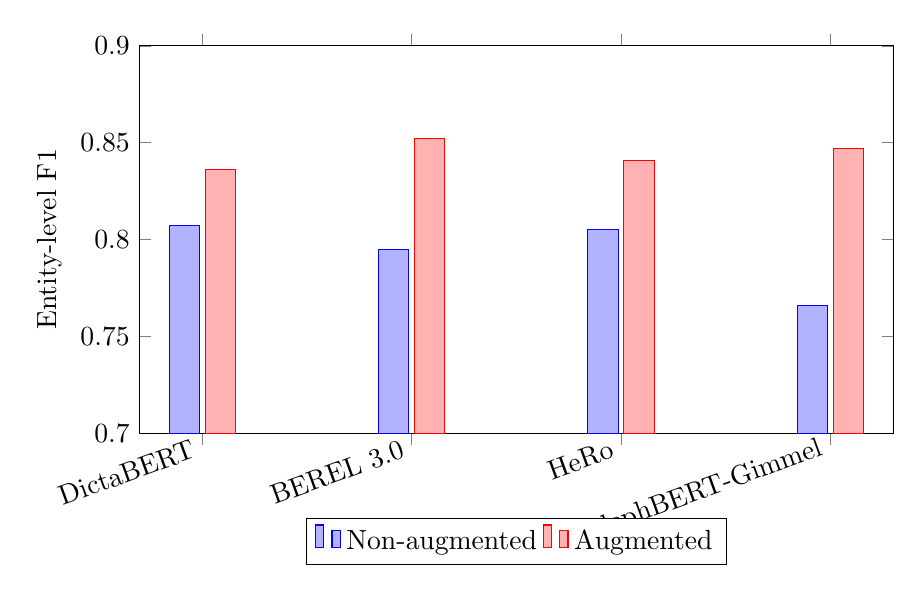
\begin{tikzpicture}
\begin{axis}[
    ybar,
    ymin=0.70,
    ymax=0.90,
    width=0.92\textwidth,
    height=6.5cm,
    ylabel={Entity-level F1},
    symbolic x coords={DictaBERT,BEREL 3.0,HeRo,AlephBERT-Gimmel},
    xtick=data,
    x tick label style={rotate=20,anchor=east},
    bar width=11pt,
    legend style={at={(0.5,-0.22)},anchor=north,legend columns=2}
]
\addplot coordinates {(DictaBERT,0.807) (BEREL 3.0,0.795) (HeRo,0.805) (AlephBERT-Gimmel,0.766)};
\addplot coordinates {(DictaBERT,0.836) (BEREL 3.0,0.852) (HeRo,0.841) (AlephBERT-Gimmel,0.847)};
\legend{Non-augmented, Augmented}
\end{axis}
\end{tikzpicture}
\caption{SVM Fusion with Multilabel Stratified split, before and after augmentation.}
\label{fig:journal_svm}
\end{figure}

Table~\ref{tab:wilcoxon_summary} summarizes the paired Wilcoxon tests. Augmentation improves all 48 matched comparisons. Multilabel stratification is especially strong in the augmented setting. SVM Fusion improves over the other reported methods in nearly all comparisons, but its router limitation should be considered when judging deployable performance.

\begin{table}[htbp]
\centering
\scriptsize
\caption{Summary of paired Wilcoxon signed-rank tests over seed-aligned runs. Positive means that the first item in the contrast improved F1.}
\label{tab:wilcoxon_summary}
\begin{tabular}{p{4.7cm}p{2.3cm}cccc}
\toprule
Contrast & Setting & Positive & Significant & Mean $\Delta$F1 & Largest $p$ \\
\midrule
Augmentation vs. same split without augmentation & All models, methods, splits & 48/48 & 48/48 & +0.085 & 3.9e-04 \\
Label-aware greedy vs. baseline random & Non-augmented & 14/16 & 10/16 & +0.021 & 0.898 \\
Multilabel stratified vs. baseline random & Non-augmented & 15/16 & 13/16 & +0.024 & 0.927 \\
Label-aware greedy vs. baseline random & Augmented & 11/16 & 13/16 & +0.009 & 0.430 \\
Multilabel stratified vs. baseline random & Augmented & 15/16 & 16/16 & +0.028 & 0.033 \\
SVM Fusion vs. Regular NER & Non-augmented & 12/12 & 12/12 & +0.073 & 8.8e-05 \\
SVM Fusion vs. Cascaded 3-step & Non-augmented & 12/12 & 12/12 & +0.071 & 2.6e-04 \\
SVM Fusion vs. Confidence Fusion & Non-augmented & 12/12 & 12/12 & +0.057 & 9.5e-06 \\
SVM Fusion vs. Regular NER & Augmented & 12/12 & 12/12 & +0.025 & 0.019 \\
SVM Fusion vs. Cascaded 3-step & Augmented & 12/12 & 12/12 & +0.023 & 0.024 \\
SVM Fusion vs. Confidence Fusion & Augmented & 12/12 & 11/12 & +0.025 & 0.076 \\
\bottomrule
\end{tabular}
\end{table}

\section{Discussion}
The results show that the final performance is not determined by the pretrained model alone. The same encoder can behave differently depending on the sentence split, the use of augmentation, and the inference pipeline. This is especially important in small corpora, where random train-test splits can be misleading.

The comparison with \citet{bengigi2025} is best understood as complementary. Their study focuses on large-scale Responsa citation-network construction. This study focuses on controlled low-resource methodology: how to split, augment, model, fuse, and test when annotation is scarce. The added value is therefore methodological rather than a direct benchmark improvement.

A practical recommendation is to avoid drawing conclusions from a single random split in this domain. A better design is to use multilabel sentence-level stratification, keep augmentation strictly within the training set, and report paired multi-seed significance tests. For deployment, the SVM router should be retrained with a separate routing-development set.

\section{Conclusion}
This paper presented a controlled study of Hebrew-Aramaic Responsa reference-component extraction as low-resource NER. The strongest robust setting uses BEREL 3.0, Multilabel Stratified splitting, targeted augmentation, and SVM Fusion, reaching 0.852 mean F1 over 20 paired seeds. A conservative non-router alternative, BEREL 3.0 with Multilabel Stratified splitting, augmentation, and Confidence Fusion, reaches 0.848. The main conclusion is that data preparation and inference design can be as important as model selection in small specialized Hebrew-Aramaic corpora.


\begin{thebibliography}{99}

\bibitem[Awasthy et~al.(2020)]{awasthy2020}
Awasthy, P., Moon, T., Ni, J., and Florian, R. (2020).
Cascaded models for better fine-grained named entity recognition.
In \emph{Proceedings of EMNLP 2020}, pages 174--184. Association for Computational Linguistics.

\bibitem[Bareket and Tsarfaty(2021)]{bareket2021nemo}
Bareket, D. and Tsarfaty, R. (2021).
Neural modeling for named entities and morphology: NEMO2.
\emph{Transactions of the Association for Computational Linguistics}, 9:909--928.

\bibitem[Beltagy et~al.(2019)]{beltagy2019scibert}
Beltagy, I., Lo, K., and Cohan, A. (2019).
SciBERT: A pretrained language model for scientific text.
In \emph{Proceedings of EMNLP-IJCNLP 2019}, pages 3615--3620.

\bibitem[Ben-Gigi et~al.(2024)]{bengigi2024viewpoint}
Ben-Gigi, N., Zhitomirsky-Geffet, M., Katzoff, B., and Schler, J. (2024).
Citation network analysis for viewpoint plurality assessment of historical corpora: The case of the medieval rabbinic literature.
\emph{PLOS ONE}, 19(7):e0307115.

\bibitem[Ben-Gigi et~al.(2025)]{bengigi2025}
Ben-Gigi, N., Zhitomirsky-Geffet, M., Schler, J., and Katzoff, B. (2025).
Automatic construction of the citation network from the medieval Jewish Responsa literature.
\emph{ACM Journal on Computing and Cultural Heritage}, 18(2):1--18.

\bibitem[Bird et~al.(2009)]{bird2009nltk}
Bird, S., Klein, E., and Loper, E. (2009).
\emph{Natural Language Processing with Python}. O'Reilly Media.

\bibitem[Chicco and Jurman(2023)]{chicco2023mcc}
Chicco, D. and Jurman, G. (2023).
The advantages of the Matthews correlation coefficient over F1 score and accuracy in binary classification evaluation.
\emph{BMC Genomics}, 24:101.

\bibitem[Cohan et~al.(2020)]{cohan2020specter}
Cohan, A., Feldman, S., Beltagy, I., Downey, D., and Weld, D. (2020).
SPECTER: Document-level representation learning using citation-informed transformers.
In \emph{Proceedings of ACL 2020}, pages 2270--2282.

\bibitem[Devlin et~al.(2019)]{devlin2019bert}
Devlin, J., Chang, M.-W., Lee, K., and Toutanova, K. (2019).
BERT: Pre-training of deep bidirectional transformers for language understanding.
In \emph{Proceedings of NAACL-HLT 2019}, pages 4171--4186.

\bibitem[Dietterich(2000)]{dietterich2000}
Dietterich, T. G. (2000).
Ensemble methods in machine learning.
In \emph{Multiple Classifier Systems}, pages 1--15. Springer.

\bibitem[Dinarelli and Rosset(2011)]{dinarelli2011}
Dinarelli, M. and Rosset, S. (2011).
Models cascade for tree-structured named entity detection.
In \emph{Proceedings of IJCNLP 2011}, pages 110--118.

\bibitem[Florian et~al.(2003)]{florian2003}
Florian, R., Ittycheriah, A., Jing, H., and Zhang, T. (2003).
Named entity recognition through classifier combination.
In \emph{Proceedings of CoNLL 2003}, pages 168--171.

\bibitem[Gueta et~al.(2023)]{gueta2023alephgimmel}
Gueta, A., Seker, A., Pereira, L., Neishtadt, E., Bandel, E., Bareket, D., Brusilovsky, I., Greenfeld, R., and Tsarfaty, R. (2023).
Large pre-trained models with extra-large vocabularies: A contrastive analysis of Hebrew BERT models and a new one to outperform them all.
\emph{arXiv:2211.15199}.

\bibitem[HaCohen-Kerner et~al.(2010)]{hacohen2010}
HaCohen-Kerner, Y., Zohar, M., and Mughaz, D. (2010).
Automatic identification of biblical quotations in Hebrew-Aramaic documents.
\emph{Cybernetics and Systems}, 41(3):180--197.

\bibitem[HaCohen-Kerner et~al.(2026)]{hacohen2026}
HaCohen-Kerner, Y., Liskovetsky, K., Mughaz, D., and Miller, D. (2026).
A comparison of advanced machine learning and deep learning methods for short text classification of Hebrew and Aramaic in Jewish Responsa.
\emph{Applied Sciences}, 16(8):3907.

\bibitem[Hu et~al.(2024)]{hu2024ner}
Hu, Q., Yu, G., Wang, X., Fukumoto, F., and Ye, Y. (2024).
A survey on deep learning for named entity recognition.
\emph{IEEE Transactions on Knowledge and Data Engineering}, 36(9):4583--4605.

\bibitem[Itai and Wintner(2008)]{itai2008}
Itai, A. and Wintner, S. (2008).
Language resources for Hebrew.
\emph{Language Resources and Evaluation}, 42:75--98.

\bibitem[Japkowicz and Stephen(2002)]{japkowicz2002}
Japkowicz, N. and Stephen, S. (2002).
The class imbalance problem: A systematic study.
\emph{Intelligent Data Analysis}, 6(5):429--449.

\bibitem[Keraghel et~al.(2024)]{keraghel2024ner}
Keraghel, I., Morbieu, S., and Nadif, M. (2024).
Recent advances in named entity recognition: A comprehensive survey and comparative study.
\emph{arXiv:2401.10825}.

\bibitem[Kohavi(1995)]{kohavi1995}
Kohavi, R. (1995).
A study of cross-validation and bootstrap for accuracy estimation and model selection.
In \emph{Proceedings of IJCAI 1995}, pages 1137--1143.

\bibitem[Lafferty et~al.(2001)]{lafferty2001crf}
Lafferty, J., McCallum, A., and Pereira, F. C. N. (2001).
Conditional random fields: Probabilistic models for segmenting and labeling sequence data.
In \emph{Proceedings of ICML 2001}, pages 282--289.

\bibitem[Li et~al.(2022)]{li2022ner}
Li, J., Sun, A., Han, J., and Li, C. (2022).
A survey on deep learning for named entity recognition.
\emph{IEEE Transactions on Knowledge and Data Engineering}, 34(1):50--70.

\bibitem[Lo et~al.(2020)]{lo2020s2orc}
Lo, K., Wang, L. L., Neumann, M., Kinney, R., and Weld, D. S. (2020).
S2ORC: The Semantic Scholar open research corpus.
In \emph{Proceedings of ACL 2020}, pages 4969--4983.

\bibitem[Ma and Hovy(2016)]{ma2016}
Ma, X. and Hovy, E. (2016).
End-to-end sequence labeling via bi-directional LSTM-CNNs-CRF.
In \emph{Proceedings of ACL 2016}, pages 1064--1074.

\bibitem[Min et~al.(2024)]{min2024plm}
Min, B., Ross, H., Sulem, E., Veyseh, A. P. B., Nguyen, T. H., Sainz, O., Agirre, E., Heinz, I., and Roth, D. (2024).
Recent advances in natural language processing via large pre-trained language models: A survey.
\emph{ACM Computing Surveys}, 56(2):Article 30.

\bibitem[Moghaz et~al.(2019)]{moghaz2019}
Moghaz, D., Zhitomirsky-Geffet, M., and HaCohen-Kerner, Y. (2019).
Text mining for Jewish scholars' birth and death years in Hebrew, Aramaic and Yiddish texts.
\emph{International Journal on Digital Libraries}, 20:197--220.

\bibitem[Mughaz et~al.(2014)]{mughaz2014}
Mughaz, D., HaCohen-Kerner, Y., and Zhitomirsky-Geffet, M. (2014).
Mining and using key-words and key-phrases to identify the era of an anonymous undated Jewish text.
\emph{Journal of Intelligent Information Systems}, 42:285--316.

\bibitem[Nguyen et~al.(2023)]{nguyen2023auc}
Nguyen, N. D., Tan, W., Du, L., Buntine, W., Beare, R., and Chen, C. (2023).
AUC maximization for low-resource named entity recognition.
In \emph{Proceedings of the AAAI Conference on Artificial Intelligence}, 37(11):13389--13399.

\bibitem[Pineau et~al.(2021)]{pineau2021}
Pineau, J., Vincent-Lamarre, P., Sinha, K., Lariviere, V., Beygelzimer, A., d'Alche-Buc, F., Fox, E., and Larochelle, H. (2021).
Improving reproducibility in machine learning research: A report from the NeurIPS 2019 reproducibility program.
\emph{Journal of Machine Learning Research}, 22:1--20.

\bibitem[Ratinov and Roth(2009)]{ratinov2009}
Ratinov, L. and Roth, D. (2009).
Design challenges and misconceptions in named entity recognition.
In \emph{Proceedings of CoNLL 2009}, pages 147--155.

\bibitem[Sade et~al.(2018)]{sade2018}
Sade, S., Seker, A., and Tsarfaty, R. (2018).
The Hebrew Universal Dependency Treebank: Past, present and future.
In \emph{Proceedings of the Second Workshop on Universal Dependencies}, pages 133--143.

\bibitem[Santoso et~al.(2024)]{santoso2024}
Santoso, J., Sutanto, P., Cahyadi, B., and Setiawan, E. (2024).
Pushing the limits of low-resource NER using LLM artificial data generation.
In \emph{Findings of the Association for Computational Linguistics: ACL 2024}.

\bibitem[Satlow and Sperling(2022)]{satlow2022}
Satlow, M. L. and Sperling, M. (2022).
The rabbinic citation network.
\emph{AJS Review}, 46(2):291--319.

\bibitem[Sechidis et~al.(2011)]{sechidis2011}
Sechidis, K., Tsoumakas, G., and Vlahavas, I. (2011).
On the stratification of multi-label data.
In \emph{Proceedings of ECML PKDD 2011}, pages 145--158. Springer.

\bibitem[Seker et~al.(2022)]{seker2022alephbert}
Seker, A., Bandel, E., Bareket, D., Brusilovsky, I., Greenfeld, R., and Tsarfaty, R. (2022).
AlephBERT: Language model pre-training and evaluation from sub-word to sentence level.
In \emph{Proceedings of ACL 2022}, pages 46--56.

\bibitem[Shalumov and Haskey(2023)]{shalumov2023hero}
Shalumov, V. and Haskey, H. (2023).
HeRo: RoBERTa and Longformer Hebrew language models.
\emph{arXiv:2304.11077}.

\bibitem[Shmidman et~al.(2022)]{shmidman2022berel}
Shmidman, A., Guedalia, J., Shmidman, S., Shmidman, C. S., Handel, E., and Koppel, M. (2022).
BEREL: BERT embeddings for rabbinic-encoded language.
In \emph{Proceedings of the Workshop on Language Technologies for Historical and Ancient Languages}, pages 49--54.

\bibitem[Shmidman et~al.(2023)]{shmidman2023dictabert}
Shmidman, A., Shmidman, S., and Koppel, M. (2023).
DictaBERT: A state-of-the-art BERT suite for Modern Hebrew.
\emph{arXiv:2308.16687}.

\bibitem[Sokolova and Lapalme(2009)]{sokolova2009}
Sokolova, M. and Lapalme, G. (2009).
A systematic analysis of performance measures for classification tasks.
\emph{Information Processing and Management}, 45(4):427--437.

\bibitem[Szymanski and Kajdanowicz(2017)]{szymanski2017}
Szymanski, P. and Kajdanowicz, T. (2017).
A network perspective on stratification of multi-label data.
In \emph{Proceedings of LID 2017}, pages 22--35. PMLR.

\bibitem[Te et~al.(2022)]{te2022}
Te, S., Barhoumi, A., Lentschat, M., Bordignon, F., Labbe, C., and Portet, F. (2022).
Citation context classification: Critical vs. non-critical.
In \emph{Proceedings of the Third Workshop on Scholarly Document Processing}, pages 49--53.

\bibitem[Tsarfaty et~al.(2019)]{tsarfaty2019}
Tsarfaty, R., Sadde, S., Klein, S., and Seker, A. (2019).
What's wrong with Hebrew NLP? and how to make it right.
In \emph{Proceedings of EMNLP-IJCNLP: System Demonstrations}, pages 259--264.

\bibitem[Webster and Kit(1992)]{webster1992}
Webster, J. J. and Kit, C. (1992).
Tokenization as the initial phase in NLP.
In \emph{Proceedings of COLING 1992}, pages 1106--1110.

\bibitem[Wei and Zou(2019)]{wei2019eda}
Wei, J. and Zou, K. (2019).
EDA: Easy data augmentation techniques for boosting performance on text classification.
In \emph{Proceedings of EMNLP-IJCNLP 2019}, pages 6382--6388.

\bibitem[Zhao et~al.(2023)]{zhao2023llm}
Zhao, W. X., Zhou, K., Li, J., Tang, T., Wang, X., Hou, Y., Min, Y., Zhang, B., Zhang, J., Dong, Z., Du, Y., Yang, C., Chen, Y., Chen, Z., Jiang, J., Ren, R., Li, Y., Tang, X., Liu, Z., Liu, P., Nie, J.-Y., and Wen, J.-R. (2023).
A survey of large language models.
\emph{arXiv:2303.18223}.

\bibitem[Zhou et~al.(2022)]{zhou2022melm}
Zhou, R., Li, X., He, R., Bing, L., Cambria, E., and Miao, C. (2022).
MELM: Data augmentation with masked entity language modeling for low-resource NER.
In \emph{Proceedings of ACL 2022}, pages 2246--2261.

\end{thebibliography}


\end{document}
